\documentclass[a4paper,12pt]{article} % добавить leqno в [] для нумерации слева

\usepackage{lab_preamble}

\begin{document}

\LabTitle{1.2.4}{Определение главных моментов инерции твердых тел с помощью крутильных колебаний}

\textbf{Цель работы}:
\begin{enumerate}
\item Измерить периоды крутильных колебаний рамки при различных положениях закрепленного в ней тела
\item Проверить теорети­ческую зависимость между периодами крутильных колебаний тела относительно различных осей
\item Определить моменты инерции относи­тельно нескольких осей для каждого тела
\item По ним найти главные моменты инерции тел и построить эллипсоид инерции
\end{enumerate}

\textbf{Приборы}:
\begin{enumerate}
\item Установка для получения крутильных колебаний (жесткая рамка, имеющая винты для закрепления в ней твердых тел, подвешенная на натянутой вертикально проволоке)
\item На­бор исследуемых твердых тел
\item Секундомер
\end{enumerate}

\section{Краткая Теория.}

$I_x,\ I_y,\ I_z$ - главные оси тела.

\begin{equation} I_x x^2 + I_y y^2 + I_z z^2 = 1. \label{eq:1} \end{equation}

\begin{figure} [h] \center
	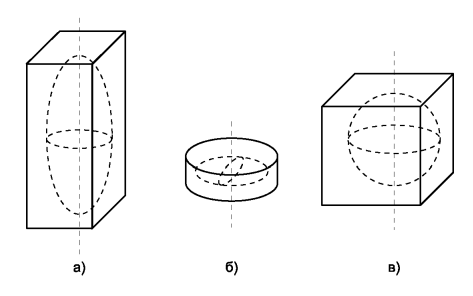
\includegraphics[scale = 1]{124/рис. 1.png}
	\label{pic:1} \caption[Рис. 1]{Эллипсоиды инерции параллелепипеда, диска и куба}
\end{figure}

\begin{equation} I = \frac{1}{r^2}. \label{eq:2} \end{equation}

\begin{figure} [h] \center 
	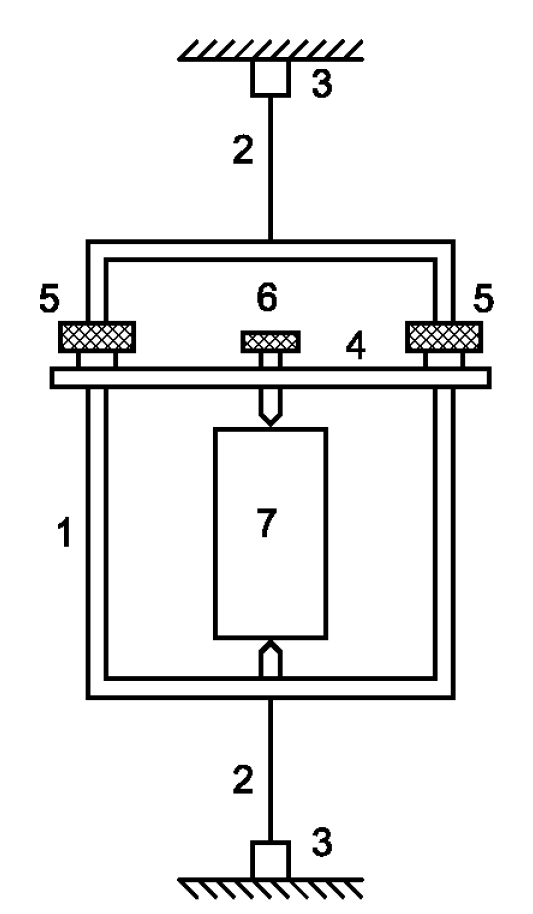
\includegraphics[scale = 0.3]{124/рис. 2.png}
	\label{pic:2} \caption[Рис. 2]{Схема установки}
	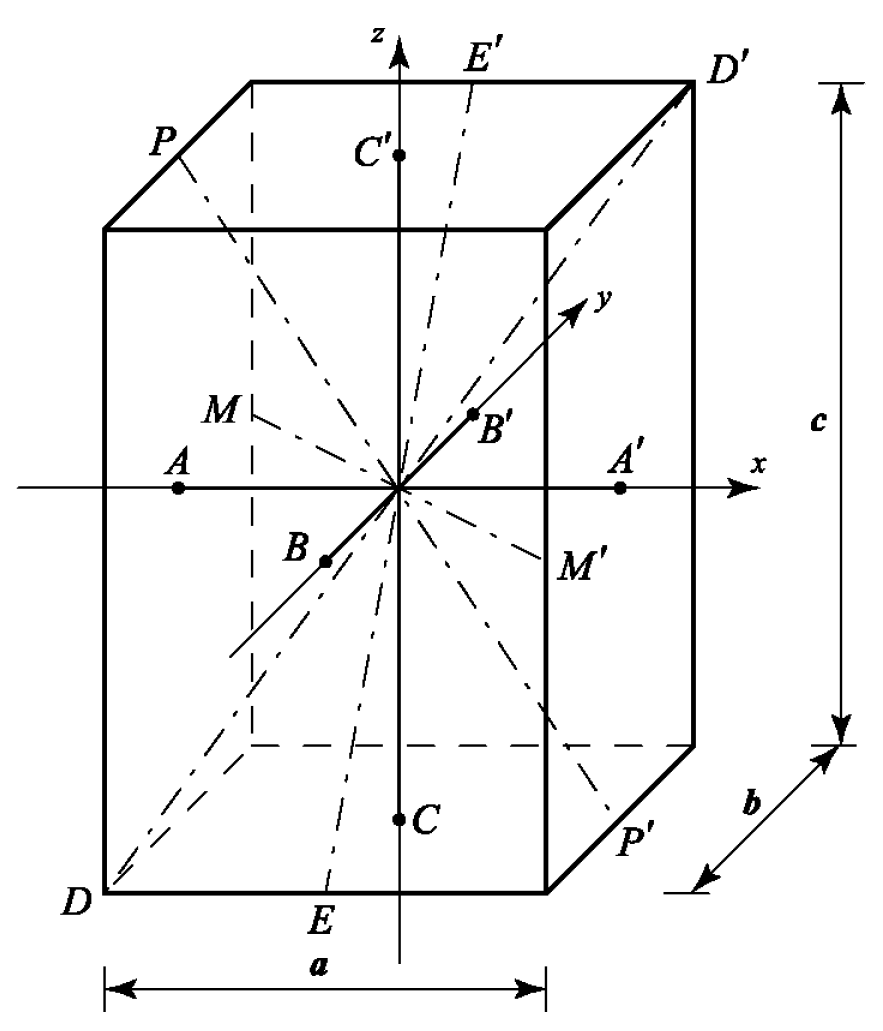
\includegraphics[scale = 0.3]{124/рис. 3.png}
	\label{pic:3} \caption[Рис. 3]{Оси вращения прямоугольного параллелепипеда}
\end{figure}

\begin{equation} (I + I_p) \frac{d^2\varphi}{dt^2} = -f\varphi. \label{eq:3} \end{equation}, где 
$I$ - момент инерции тела, 
$I_p$ - момент инерции установки, 
$\varphi$ - угол отклонения рамки, 
$f$ - модуль кру­чения проволоки.

\begin{equation} T = 2\pi \sqrt{\frac{I+I_p}{f}}. \label{eq:4} \end{equation}


\begin{equation} I_d = I_x \frac{a^2}{d^2} + I_y \frac{b^2}{d^2} + I_z \frac{c^2}{d^2}. \label{eq:5} \end{equation}
\begin{equation} \eqref{eq:5} \implies I_d (a^2 + b^2 + c^2) = I_x a^2 + I_y b^2 + I_z c^2. \label{eq:6} \end{equation}
\begin{equation} \eqref{eq:4} \implies T_d (a^2 + b^2 + c^2) = T_x a^2 + T_y b^2 + T_z c^2. \label{eq:7} \end{equation}
\begin{equation} (b^2 + c^2)T_E^2 = b^2 T_y^2 + c^2 T_z^2. \label{eq:8} \end{equation}
\begin{equation} (a^2 + c^2)T_P^2 = a^2 T_x^2 + c^2 T_z^2. \label{eq:9} \end{equation}
\begin{equation} (a^2 + b^2)T_M^2 = a^2 T_x^2 + b^2 T_y^2. \label{eq:10} \end{equation}

\section{Выполнение.}
\begin{enumerate}
\item Ознакомимся с установкой для получения крутильных колебаний. Проверим: 1) хорошо ли натянута проволока, 2) жестко ли закреплена на ней рамка, 3) нормально ли работает устройство для возбуждения крутильных колебаний, 4) не возникают ли, кроме крутильных колеба­ний рамки, еще и колебания в вертикальной плоскости (их не должно быть).

\item Научимся закреплять тела в рамке. На телах имеются специальные углубления, в которые должны входить винты, имеющиеся на рамке. Отвернув гайки 5, под­нимим вверх подвижную планку 4 на рамке, вставим тело в рамку, попав углублением, имеющимся на теле, на выступ нижней стороны рамки. Опуская планку, необходимо выступающим из планки на 5-7 мм вин­том 6 попасть в отверстие на теле. Закрепив планку гайками 5, немного подожмем тело винтом 6. Если в дальнейшем обнаружится, что тело поворачивается в рамке, надо его еще поджать винтом 6.

\item Перед каждой серией измерений необходимо выбрать амплитуду крутильных колебаний.

\item Для рамки со всеми телами при различных их положениях определим периоды колебаний по времени 10-15 колебаний, повторяя каждое измерение не менее 3 раз. (см т. 1)
\begin{table} [h]
\center

\begin{tabular}{l|l|lllll}
&&измерения, T, с&&&&\\
\hline
тело&ось&1&2&& \textless T \textgreater, с&I\\
\hline
установка&&2.581&2.572&& 2.58 &\\
куб&z&3.097&3.088&& 3.09 &7.81E-04\\
&xy&3.085&3.082&& 3.08 &7.81E-04\\
&xyz&3.097&3.085&& 3.09 &7.81E-04\\
параллелипипед&x&3.825&3.828&& 3.83 &4.35E-03\\
&y&4.122&4.199&& 4.16 &5.65E-03\\
&z&3.285&3.272&& 3.28 &2.19E-03\\
&MM'&3.885&3.884&& 3.88 &4.64E-03\\
&PP'&3.475&3.469&& 3.47 &3.02E-03\\
&EE'&3.381&3.372&& 3.38 &2.74E-03\\
&DD'&3.512&3.512&& 3.51 &3.29E-03\\
цилиндр 1&z&3.496&3.491&& 3.49 &3.04E-03\\
&x&3.087&3.091&& 3.09 &1.56E-03\\
цилиндр 2&z&3.268&3.256&& 3.26 &1.43E-03\\
&x&3.072&3.081&& 3.08 &1.17E-03\\

\label{tab:1}

\end{tabular}
\caption[Таблица 1]{Измерения}
\end{table}

\item Штангенциркулем измерим геометрические размеры параллелепипе­да (a, b и c). Вычислим главные моменты инерции. По полученным ранее дан­ным проверим справедливость формул \eqref{eq:7} - \eqref{eq:10}. \\
\eqref{eq:7}: ошибка - $0,03\%$ \\
\eqref{eq:8}: ошибка - $0,1\%$ \\
\eqref{eq:9}: ошибка - $0,9\%$ \\
\eqref{eq:10}: ошибка - $0,6\%$ \\

\item  Нарисуем  сечения  эллипсоида  инерции  главными  плоскостями.  Для этого  выберите  измеренные  периоды колебаний  для  осей  в  главной плоскости и для каждой оси вычислите величину $\frac{1}{\sqrt{T^2 - T_p^2}}$, которая пропорциональна расстоянию  от  центра масс  тела до точки  пересече­ния эллипсоида с этой осью.  Эти величины надо отложить вдоль направлений соот­ветствующих осей (должно получиться 8 точек) и через их концы про­вести  эллипс.  Это и будет  сечение  эллипсоида главной  плоскостью  (в произвольном масштабе). \ref{pic:4}

\item Проведем аналогичные измерения для куба и построим для него соот­ветствующие сечения эллипсоида инерции. Убедимся в равенстве всех центральных моментов инерции. \ref{pic:5}

\newpage

\begin{figure} [h] \center
	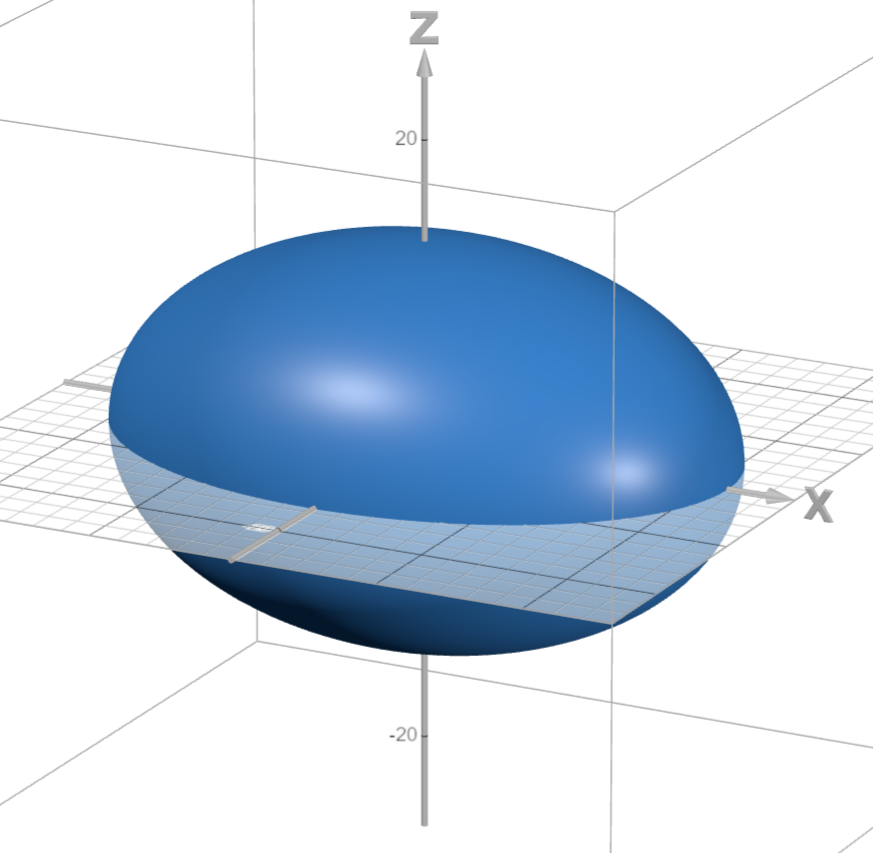
\includegraphics[scale=0.5]{./124/elipse.png}
	\label{pic:4} \caption[Рис. 4]{Эллипсоид инерции параллелепипеда}
	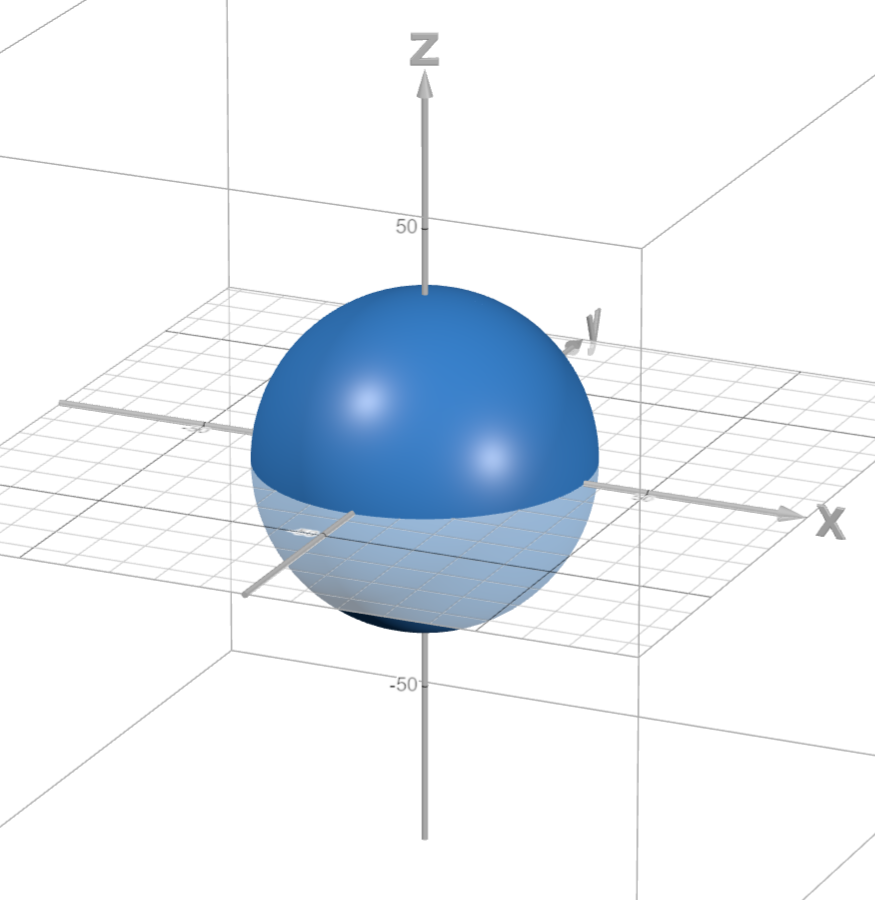
\includegraphics[scale=0.5]{./124/elipse 2.png}
	\label{pic:5} \caption[Рис. 5]{Эллипсоид инерции куба}
\end{figure}



\item Построим график зависимости $T^2$ от $I$ и убедимся в его линейности. \ref{pic:6}

\newpage

\begin{figure} [h] \center
	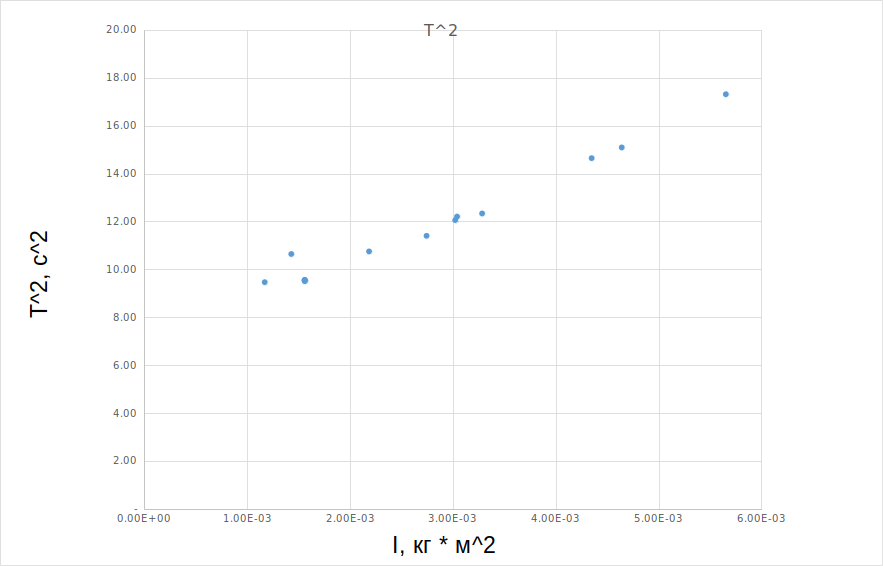
\includegraphics[scale=0.5]{124/graph.png}
	\label{pic:6} \caption[Рис. 6]{График зависимости $T^2(I)$}
\end{figure}

\section{Вывод}
В ходе данной лабораторной работы мы измерили периоды крутильных колебаний рамки при различных положениях закрепленного в ней тела, проверили теоретическую зависимость между периодами колебаний параллелепипеда относительно различных осей, определили моменты инерции тел относительно нескольких осей и построили эллипсоиды инерции.

\end{enumerate}

\end{document}